% Template for Cogsci submission with R Markdown

% Stuff changed from original Markdown PLOS Template
\documentclass[10pt, letterpaper]{article}

\usepackage{cogsci}
\usepackage{pslatex}
\usepackage{float}
\usepackage{caption}

% amsmath package, useful for mathematical formulas
\usepackage{amsmath}

% amssymb package, useful for mathematical symbols
\usepackage{amssymb}

% hyperref package, useful for hyperlinks
\usepackage{hyperref}

% graphicx package, useful for including eps and pdf graphics
% include graphics with the command \includegraphics
\usepackage{graphicx}

% Sweave(-like)
\usepackage{fancyvrb}
\DefineVerbatimEnvironment{Sinput}{Verbatim}{fontshape=sl}
\DefineVerbatimEnvironment{Soutput}{Verbatim}{}
\DefineVerbatimEnvironment{Scode}{Verbatim}{fontshape=sl}
\newenvironment{Schunk}{}{}
\DefineVerbatimEnvironment{Code}{Verbatim}{}
\DefineVerbatimEnvironment{CodeInput}{Verbatim}{fontshape=sl}
\DefineVerbatimEnvironment{CodeOutput}{Verbatim}{}
\newenvironment{CodeChunk}{}{}

% cite package, to clean up citations in the main text. Do not remove.
\usepackage{apacite}

% KM added 1/4/18 to allow control of blind submission


\usepackage{color}

% Use doublespacing - comment out for single spacing
%\usepackage{setspace}
%\doublespacing


% % Text layout
% \topmargin 0.0cm
% \oddsidemargin 0.5cm
% \evensidemargin 0.5cm
% \textwidth 16cm
% \textheight 21cm

\title{Analyzing contingent interactions in R with \texttt{chattr}}


\author{{\large \bf Marisa Casillas (mcasillas@uchicago.edu)} \\ Comparative Human Development, 1101 E. 58th St. \\ Chicago, IL 60637 USA \AND {\large \bf Camila Scaff (camiscaff@hotmail.com)} \\ Department, Address \\ Zurich, Switzerland POSTCODE}


\begin{document}

\maketitle

\begin{abstract}
Include no author information in the initial submission, to facilitate
blind review. The abstract should be one paragraph, indented 1/8 inch on
both sides, in 9\textasciitilde point font with single spacing. The
heading `Abstract' should be 10\textasciitilde point, bold, centered,
with one line of space below it. This one-paragraph abstract section is
required only for standard six page proceedings papers. Following the
abstract should be a blank line, followed by the header `Keywords' and a
list of descriptive keywords separated by semicolons, all in
9\textasciitilde point font, as shown below.

\textbf{Keywords:}
Add your choice of indexing terms or keywords; kindly use a semi-colon;
between each term.
\end{abstract}

\hypertarget{introduction}{%
\section{Introduction}\label{introduction}}

The current paper introduces an R (REFS) package called \texttt{chattr}
that facilitates the detection and analysis of temporally contingent
interactions in pre-annotated data
(\href{}{https://github.com/marisacasillas/chattr-basic}).\footnote{At
  time of submission, the conversion from R scripts to R package is
  still underway. That said, all documentation, scripts, and tests are
  available at the given URL. The fully packaged version will be
  available at the same URL (minus ``-basic'') before May 2021.} Current
tools for conducting similar analyses from annotated data are either
proprietary, thereby limiting access to potential users, or constructed
ad-hoc, thereby introducing significant variation in the constructs
being measured across studies. The \texttt{chattr} package aims to
improve this situation in two ways: (1) It takes inspiration from the
fields of conversation analysis, psycholinguistics, and language
development to provide flexible but theoretically sound measurements of
temporally contingent interaction at scale and (2) its open-source
toolkit accepts a handful of generic formats as input, opening up its
analytical framework to a wide variety of domains (e.g., child language
input, multi-party adult conversation, non-human animal signal
exchanges, multi-modal contingencies produced by a single organism,
etc.). The remainder of this short report reviews the theoretical basis
underlying the development of \texttt{chattr}, describes the core
functions offered by the package, and demonstrates its use in three
existing datasets.

\hypertarget{contingent-interaction}{%
\subsection{Contingent interaction}\label{contingent-interaction}}

The joint coordination of action by two or more agents usually involves
temporal contingencies. Whether we are making music with others,
crossing a busy intersection, or chatting with a friend, the timing of
our contributions to a coordinated event is crucial to its success. In
many cases, the optimal strategy for coordination involves some form of
turn taking. In a typical turn-taking interaction, only one interactant
makes their contribution at a time, and decisions about who contributes
when can be determined flexibly (as in conversation) or in a pre-defined
manner (as in a debate). This sequential structure enables interactants
to adapt each contribution such that it relevantly progresses the joint
activity and to initiate unplanned subsequences (e.g., repairing a
misunderstanding) without breaking from moving toward the the larger
goal.

Turn-taking interactions, or temporally contingent interactions that
appear much like them, are used for communication across the animal
kingdom (REFS). In humans, turn-taking interactions may be the only
reliable source of language universals (REFS). Traditionally, these
kinds of interactional contingencies have been studied using careful
inspection and analysis (both qualitative and quantitative) of manual
measurements from video and audio recordings. However, recent advances
in automated annotation tools (e.g., tools for vocalization detection)
have opened up the possibility to investigate interactional behavior at
a much larger scale, creating a need for new and validated analytical
approaches.

\hypertarget{tools-for-contingency-detection-and-their-shortcomings}{%
\subsection{Tools for contingency detection (and their
shortcomings)}\label{tools-for-contingency-detection-and-their-shortcomings}}

At present, the most widely used tool with respect to automated
contingency analysis of human interaction is the LENA system (REFS).
LENA is meant to be used with young children, but can also be used to
capture adult language environments (REFS). The system includes both a
recording device and a set of proprietary software tools that enable the
researcher to first collect long-format (16-hour) participant-centric
audio recordings and then, second, automatically analyze them for a
range of properties, such as when vocalizations occur by speakers of
different types (e.g., near and far female adult vocalizations). The
software then uses the detected vocalizations to find candidate regions
of vocal exchange (VABs; Vocal Activity Blocks) between the target child
and nearby adults. It then calculates the estimated number of speaker
exchanges that involve the child, using temporal contingency to
associate speaking turns from different speaker types (i.e., \textless5
seconds of silence between child and woman/man vocalizations or vice
versa). Turn-taking information is provided both in summary form (i.e.,
the CTC; Conversational Turn Count) and as vocalization metadata in
their derived output file (``.its'' file).

This extremely convenient system, which has been critical to spurring
new research on language development and turn-taking in recent years
(REFS), also has a few unfortunate drawbacks. Validation studies show
reliability estimates for CTC between 0.3 and 0.6 (REFS; Bulgarelli et
al., under review; Cristia et al., under review), with systematically
worse errors for younger infants than older ones (REFS).\footnote{Note
  that most CTC error estimates inherit error from earlier steps in the
  processing pipeline (e.g., misidentifying the speech as silence).} The
LENA system is also proprietary, fairly expensive, and can only be used
with recordings made with the LENA device. Therefore, research groups
who lack generous funding or who have special hardware and storage
requirements will struggle to benefit from the system. Lastly, LENA is
designed specifically to work for child wearers. While this benefits the
accuracy of its applciation in the child home language context, it means
that the output, particularly the CTC measures have little utility for
those interested in adult-centric audio or even vocal and multi-modal
exchanges between non-human animals.

Outside of the LENA context, approaches to extracting temporal
contingencies over whole corpora have been much more variable. For
example, in studies of adult conversation, researchers vary in what
timing windows qualify as contingent, what types of contributions count
toward turn taking, the modality in which communication is taking place,
in how many interactants are considered to be involved (or are of
particular interest), and so on, as is suitable to the research question
(REFS; Roberts et al (2015) Heldner \& Edlund? Bosch Animal studies??).
These studies, while heterogenous in data types and precise analytical
decisions about how and when to count turn-taking exchanges, have
typically been inspired by core concepts from conversation analysis,
building up significant theoretical common ground for understanding
moment-to-moment processes of interactant coordination. Much of the work
on language development, by contrast, has inherited the somewhat
idiosyncratic concepts and terminology introduced by the LENA system,
leaving a conceptual disjunct between work on turn-taking behaviors in
children, adults, and non-human animals.

Given the various restrictions on existing tools and free variations in
analysis across studies, there is a clear need for a free, flexible, and
theoretically grounded tool that can extract temporal contingencies at
scale; \texttt{chattr} aims to fill this need. The following text
briefly describes the package and its use before turning to examples
with real datasets.

\hypertarget{the-chattr-system}{%
\section{\texorpdfstring{The \texttt{chattr}
system}{The chattr system}}\label{the-chattr-system}}

In brief, \texttt{chattr} is an R package that gives both detailed and
summary data on temporal contingencies in pre-annotated interactional
data of the user's choice. To keep things simple, it has a single core
function for each type of input that it takes: (a) LENA .its files; (b)
tab delimited .txt tables with one utterance per row, as can be exported
from Praat, ELAN, and so forth (REFS); and (c) .rttm tables, a common
output format used with automated speech diarization systems.\footnote{Users
  interested in a fully open-source pipeline for child language
  environments should check out Lavechin et al.'s (REFS) voice type
  classifier.} Users can use the default settings for each function, or
can customize as desired. More advanced users can capitalize on the wide
variety of sub-functions utilized by the core input-type functions. All
settings, output information types, and theoretical background is
thoroughly summarized in the online documentation where the project is
stored on GitHub.

\hypertarget{core-concepts-and-default-settings}{%
\subsubsection{Core concepts and default
settings}\label{core-concepts-and-default-settings}}

Before employing \texttt{chattr}, users should review how it employs
concepts of `turn', `transition', and `interactional sequence' since
these differ from those typically used in the language development
literature and are somewhat restricted interpretations of their full
(and human conversation-specific) theoretical meanings in conversation
analysis (e.g., see REFS). We briefly summarize these core concepts
here. The same concepts are illustrated in Figure 1. We use the concepts
of `producer' and `recipient'/`addressee' rather than `speaker' and
`listener' to underscore the utility of these concepts across
modalities, species, and interactional contexts:

\emph{`Turns'} are conceived of as one or more closely occurring
vocalizations by the same producer. Distinct from an utterance, a turn
can be formed of multiple complete communicative acts that may be
separated by pauses in production so long as (a) there is no intervening
other producer who begins before the next increment of production begins
and (b) the pause in production is short. An example of a single-unit
turn in English is ``Jane is the one in the hat.''. An example of a
multi-unit turn in English is ``Jane is the one in the hat- third from
the left, see?''.

\emph{`Turn transitions'} occur when one producer's turn stops and
another producer's turn begins. Every turn transition has a
pre-transition producer and a post-transition producer---these must be
different speakers. The transition \emph{begins} when the first turn
ends and \emph{ends} when the second turn starts. Therefore, if the
second turn starts before the first turn ends, the transition time is
negative; this is referred to as an instance of `transitional overlap'.
If the second turn starts after the first turn ends, the transition time
is positive; referred to as an instance of `transitional gap'.

\emph{`Interactional sequences'} are unbroken sequences of turn taking
between the target interactant and one or more of their interactional
partners. Interactional sequences may reflect more structurally complex,
engaged interactional behaviors than single turn transitions do.
Interactional sequences may be more akin to conversational bouts, in
which participants can more substantially build on joint goals than in
single transitional exchanges alone.

\begin{CodeChunk}
\begin{figure*}[h]

{\centering 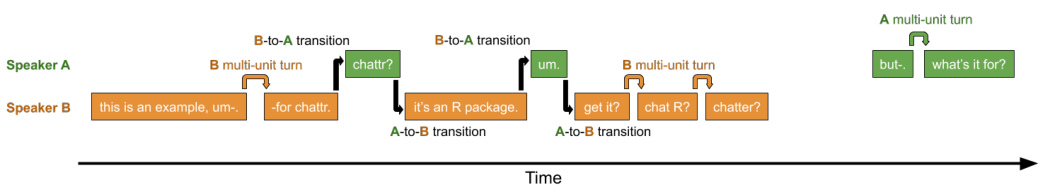
\includegraphics{figs/minisequence-1} 

}

\caption[An example of a brief dyadic interaction between two English speakers]{An example of a brief dyadic interaction between two English speakers: A (green) and B (orange). The producers here use both single- and multi-unit turns. There are 6 turns (3 from each producer), 4 turn transitions (two each from B to A and vice versa; black arrows), and one interactional sequence (the contiguous block of producer continuation/transition marked with green/orange arrows; the other turn ('but-. what's it for?') has no transitions and so is not an interactional sequence):}\label{fig:minisequence}
\end{figure*}
\end{CodeChunk}

\hypertarget{default-settings}{%
\subsubsection{Default settings}\label{default-settings}}

The default settings are designed for human spontaneous conversation,
which demonstrates fairly robust timing patterns across the diverse
collection of signed and spoken languages previously analyzed (REFS).
Note that young children's contingent responses are slower than adults'
(REFS) but that timing is also considered in the default settings, which
give a generous analysis window.

In brief, the three default settings that influence turn-taking outcomes
are that: (a) up to 2000 ms of transitional gap or up to 1000 ms of
transitional overlap is allowed between turns in detecting turn
transitions between producers, (b) turn transitions can occur with turns
of any duration, type, and between any potential interactional partner
and the target interactant (the latter must usually be specified by the
user), and (c) when there are multiple potential prompts or responses to
a turn, \texttt{chattr} picks the turn that begins soonest after the
current turn. The LENA input function \texttt{fetch\_chatter\_LENA()}
has several additional defaults that partly emulate LENA's CTC measure:
That is, the target producer is ``CH'', potential interactants are
``FA'' and ``MA'', and transitions are only counted if the associated
turns contain some linguistic material (REFS).

\hypertarget{example-use-cases}{%
\subsubsection{Example use cases}\label{example-use-cases}}

Suppose that I am interested in studying child-child interactions using
LENA data. I would first collect the LENA .its files of interest (e.g.,
from HomeBank or from my own source) into a local directory on my
computer. Then I would use \texttt{fetch\_chatter\_LENA()} with each
file, but I would change the default interactants to include only ``OC''
(i.e.~any non-target-child vocalization), remove the requirement for
turns to have linguistic content (which is not automatically estimated
for other children in LENA's output), and specify my interest in nearby
interactants only (i.e., not ``far'' detected vocalizations). This
customized call,
\texttt{fetch\_chatter\_LENA(filename,\ interactants\ =\ "OC",\ default.lxonly\ =\ FALSE,\ nearonly\ =\ TRUE)}
would then return a table that shows, for each target child vocalization
in each .its file, what other vocalizations it was grouped with into
turns, which vocalizations from other children were detected as possible
prompts and responses to target child vocalizations, and the grouping of
those target child vocalizations and their prompts and responses into
interactional sequences. For each file I would also get a second table
that gives overall descriptive statistics about turns, transitions, and
interactional sequences for that file. From these tables I could conduct
tests of my hypotheses about child-child interactions (e.g., they
increase in frequency and duration with age; REFS) and plot the results.

Suppose instead that I am interested in investigating how adult
conversational patterns vary across structured cooperative contexts
(e.g., at different phases during board games). I would first find a
dataset with both utterance and game phase annotations (or recordings of
games that I could annotate by hand or using an automated tool). I would
ensure that the annotations are formatted as a tab-delimited text file
as specified in the \texttt{chattr} documentation. Then I would use the
most general call, \texttt{fetch\_chatter\_BST()} (BST stands for Basic
Speech Table) to fetch turn-taking information across the recording.
Perhaps I am interested in a minimum utterance duration and a more
strict temporal window for contingency (all expressed in milliseconds).
I might also want to calculate 10 randomized simulations of turn-taking
rates as a sanity check for how many of the detected transitions are
spurious. I would then customize the function call accordingly before
using it over each file, as in
\texttt{fetch\_chatter\_BST(filename,\ min.utt.dur\ =\ 1500,\ allowed.gap\ =\ 1000,\ allowed.overlap\ =\ 600,\ n.runs\ =\ 10)}.
As in the previous example, this call should result in tables of
turn-taking behavior that could be used in conjunction with my
annotations of game phase to test my hypotheses.

\hypertarget{limitations}{%
\subsection{Limitations}\label{limitations}}

Any analyst looking manually at interactional data would always first
check that the speakers are indeed mutually engaged before labeling
and/or measuring an observed interactional phenomenon for further
analysis (e.g., child-to-other turn transition). Unfortunately, this
rich criterion for \emph{semantic} contingency between turns---not just
\emph{temporal} contingency---is beyond what \texttt{chattr} can do.
Consider, for example, a case where four co-present speakers engage in
two simultaneous conversations. Because \texttt{chattr} only looks for
temporal contingencies, it may detect transitions across conversations,
and at the expense of catching within-conversation transitions. It is
important to remember that \texttt{chattr} only detects temporal
patterns that \emph{look like} turn-taking behavior. You as the analyst
are responsible for checking how reliably the detected turn-taking
behavior alighns with true conversational interaction behavior. To
overcome this limitation, consider adding addressee coding when your
data features simultaneous interactions and/or highly variable
interactional contexts.

\hypertarget{references}{%
\section{References}\label{references}}

\setlength{\parindent}{-0.1in} 
\setlength{\leftskip}{0.125in}

\noindent

\bibliographystyle{apacite}


\end{document}
